% Provenance (never printed): see sources/outline_sources.md (Year 2: anatexis, migmatites,
% granite types and their sources). Wet granite solidus from Stern and Wyllie (1981) and
% Boettcher and Wyllie (1968); dehydration-melting brackets from Patino Douce and Harris
% (1998), Berger and Kalt (1999), Skjerlie and Johnston (1996); water solubility from Holtz
% et al. (1995); migmatite terms from the IUGS-SCMR proposal and BGS RR 99-02; aluminosity
% after Shand (as given by Moyen et al. 2017); figure data in figdata/bachelor-2/anatexis.py
% (paths from ptpaths.py); exercise and problem values in the Book 4 scratch calculator
% calc/ch12.py.
\chapter{A fusão da crosta: migmatitos e granitos}\label{ch:b2:crustal-melting}

O granito é o que torna os continentes leves, e o manto não pode produzi-lo diretamente: os
fundidos do \omterm{def:b2:mantle-melting:peridotites}{peridotito} são basaltos. A maior parte do granito é a crosta continental fundindo a si mesma.
Quando uma raiz de montanha espessada se aquece, quando um basalto se acumula sob a crosta, ou quando uma rocha
quente sobe e sua pressão cai, as micas e os anfibólios da crosta profunda cedem
sua água, um líquido granítico aparece entre os grãos, e a rocha se torna um
\omterm{def:b2:crustal-melting:migmatite}{migmatito}, meio metamórfico, meio ígneo. Este capítulo segue esse líquido de suas primeiras
películas até o \omterm{def:b2:magma-emplacement:bodies}{plúton} que ele pode construir, e lê na química de um granito a rocha da qual ele
veio.

\begin{recall}
\textbf{Do volume do ensino médio}: granito, granitoide e granodiorito; rochas félsicas e máficas;
as raízes das cadeias de montanhas. \textbf{Do volume do primeiro ano}: a produção de calor radiogênico
na crosta; a hidrólise dos silicatos e os argilominerais. \textbf{Dos livros de química}: o solidus e o liquidus
de um sistema binário, a massa molar e a quantidade de matéria. \textbf{Do
\cref{ch:b2:magma-emplacement}}: \omterm{def:b2:magma-emplacement:bodies}{diques}, \omterm{def:b2:magma-emplacement:bodies}{plútons} e \omterm{def:b2:magma-emplacement:ascent}{diápiros}. \textbf{Do
\cref{ch:b2:mantle-melting}}: \omterm{def:b2:mantle-melting:melting}{fusão parcial}, \omterm{def:b2:mantle-melting:peritectic}{fusão incongruente} e \omterm{def:b2:mantle-melting:melting}{fusão por
descompressão}. \textbf{Do \cref{ch:b2:metamorphic-facies}}: \omterm{def:b2:metamorphic-facies:protoliths}{metapelitos}, \omterm{def:b2:metamorphic-facies:clapeyron}{inclinação de Clapeyron} de
uma reação e fácies. \textbf{Do \cref{ch:b2:pt-paths}}: \omterm{def:b2:pt-paths:ptt}{trajetórias P--T--t} e o
modelo de espessamento da crosta.
\end{recall}

\section{Por que a crosta funde}\label{sec:b2:crustal-melting:why}

A palavra para isso é antiga e simples.

\begin{definition}[Anatexia]\label{def:b2:crustal-melting:anatexis}
A \emph{anatexia}\index{anatexia} é a fusão de uma rocha, qualquer que seja o grau de fusão;
na prática, a palavra é usada para a \omterm{def:b2:mantle-melting:melting}{fusão parcial} da crosta continental.
\end{definition}
% ledger: scmr:migmatite

\subsection*{O solidus úmido}

O granito só funde a baixa temperatura quando está úmido. Stern e Wyllie fundiram um granito
a biotita do \omterm{def:b2:magma-emplacement:bodies}{batólito} de Sierra Nevada com excesso de água: o primeiro líquido apareceu a
\qty{680}{\celsius} a \qty{2}{kbar} e a \qty{620}{\celsius} a \qty{10}{kbar}, e a
rocha inteira só estava fundida \qty{35}{\celsius} acima do solidus a \qty{2}{kbar}, mas
\qty{105}{\celsius} acima dele a \qty{10}{kbar}. O mesmo granito, estudado antes por
Boettcher e Wyllie, começou a fundir a \qty{605}{\celsius} a \qty{15.3}{kbar}; perto de
\qty{17}{kbar}, seu plagioclásio se decompôs em jadeíta e quartzo, e a partir daí o solidus
voltou a subir, chegando a \qty{670}{\celsius} a \qty{27}{kbar}.
% ledger: sw81:wet-solidus, bw68:wet-solidus

O solidus úmido cai à medida que a pressão sobe, o contrário de um solidus seco. A razão está em para onde
vai a água. A água livre é um fluido de baixa densidade; dissolvida no fundido, ela ocupa muito
pouco espaço: Holtz e colaboradores encontraram para seu volume molar parcial em um fundido granítico valores próximos
de \qtyrange{10}{12}{\cubic\centi\metre\per\mole}, contra \qty{18}{\cubic\centi\metre\per\mole}
para a água líquida em condições ambientes, e mais para um fluido quente. A reação de fusão
\[\text{quartzo} + \text{feldspatos} + \ce{H2O}\ (\text{fluido}) \longrightarrow
\text{fundido hidratado}\]
tem portanto uma variação de volume negativa, enquanto sua variação de entropia, como em toda fusão, é
positiva: pela relação de Clapeyron do \cref{ch:b2:metamorphic-facies}, sua inclinação
$\mathrm{d}P/\mathrm{d}T = \Delta S/\Delta V$ é negativa. A pressão também deixa entrar mais água
no fundido: para um fundido haplogranítico a \qty{800}{\celsius}, o teor de saturação sobe
de \qty{2.80}{\percent} em massa a \qty{0.5}{kbar} para \qty{9.97}{\percent} a
\qty{5}{kbar} e \qty{13.82}{\percent} a \qty{8}{kbar}, cerca de \qty{1.27}{\percent} a mais
por quilobar entre 3 e \qty{8}{kbar}.
% ledger: holtz95:solubility

\begin{omfigure}
\centering
\begin{tikzpicture}
\begin{axis}[omrecord, width=0.5\linewidth, height=4.8cm,
  xmin=0, xmax=9, ymin=0, ymax=15, xlabel={$P$ (\unit{kbar})},
  ylabel={\ce{H2O} no fundido (\unit{\percent})},
  tick label style={font=\scriptsize}, label style={font=\small}]
\addplot[only marks, mark=*, mark size=1.6pt, blue!70!black]
  table[x=P_kbar, y=H2O_wt] {figdata/out/bachelor-2-anatexis-water.dat};
\addplot[thick, red!75!black] table[x=P_kbar, y=H2O_wt] {figdata/out/bachelor-2-anatexis-waterfit.dat};
\end{axis}
\end{tikzpicture}
\par\smallskip{\small Água que um fundido haplogranítico pode dissolver a \qty{800}{\celsius}
(pontos medidos); em vermelho, a reta de mínimos quadrados pelos pontos de 3 a
\qty{8}{kbar}, de inclinação \qty{1.26}{\percent} por quilobar.}
\end{omfigure}
% ledger: holtz95:solubility

Mas a crosta profunda contém pouca água livre: uma rocha metamórfica que foi aquecida já
expulsou a maior parte de sua água de poros, pelas reações de desidratação do
\cref{ch:b2:metamorphic-facies}. Sua água está agora presa nas micas e nos anfibólios. A fusão
precisa então esperar que esses próprios minerais se decomponham.

\begin{definition}[Fusão com fluido e fusão por desidratação]\label{def:b2:crustal-melting:reactions}
A \emph{fusão com fluido}\index{fusão com fluido} (ou fusão por influxo de água) é a
fusão na presença de um fluido aquoso livre, no solidus úmido ou perto dele; o fundido
produzido é limitado pelo suprimento de fluido. A \emph{fusão por desidratação}\index{fusão por desidratação}
(fusão sem fluido) é a \omterm{def:b2:mantle-melting:peritectic}{fusão incongruente} de um mineral hidratado, mica ou
anfibólio, com quartzo e feldspato, sem nenhum fluido livre: a água do mineral
entra no fundido, e novos minerais anidros (feldspato potássico peritético, aluminossilicato,
granada, cordierita, ortopiroxênio) crescem ao lado dele.
\end{definition}
% ledger: pj98:productivity, koester02:melting, pdh98:himalaya

Os experimentos fixam onde cada mineral hidratado cede. Em muscovita-xistos do
Himalaia, Patiño Douce e Harris encontraram uma \omterm{def:b2:crustal-melting:reactions}{fusão por desidratação} que começava a 750 a
\qty{800}{\celsius} entre 6 e \qty{10}{kbar}; a água acrescentada às mesmas rochas abaixou o
solidus, mas deu fundidos trondhjemíticos diferentes dos \omterm{def:b2:crustal-melting:leucogranite}{leucogranitos}. Um gnaisse semipelítico
começou a fundir perto de \qty{700}{\celsius} por meio de sua muscovita fengítica, mas produziu menos
de \qty{9}{\percent} de fundido; acima de \qty{800}{\celsius}, a decomposição da biotita e da
cordierita deu de 10 a \qty{63}{\percent} em volume. A \omterm{def:b2:crustal-melting:reactions}{fusão por desidratação} da biotita ocorreu
a 800 a \qty{850}{\celsius} e 0.5 a \qty{0.7}{GPa} nos \omterm{def:b2:crustal-melting:migmatite}{migmatitos} da
Floresta da Baviera, e o anfibólio acrescenta cerca de \qty{25}{\percent} de fundido em volume entre 875
e \qty{925}{\celsius} a 10 a \qty{12.5}{kbar}. A ordem é a da força com que a água é retida:
a muscovita primeiro, a biotita em seguida, o anfibólio por último.
% ledger: pdh98:himalaya, koester02:melting, bk99:migmatites, sj96:amphibole, moyen17:aluminosity

\begin{proposition}[Uma fração de fundido limitada pela água]\label{prop:b2:crustal-melting:water}
Na \omterm{def:b2:crustal-melting:reactions}{fusão por desidratação} sem nenhum fluido livre, se uma rocha contém uma fração em massa $X$ de um
mineral hidratado que contém uma fração em massa $w$ de água, e se toda essa água entra em um
fundido que contém uma fração em massa $c$ de água, a fração em massa de fundido é
\[F = \frac{X\,w}{c}.\]
Como $c$ não pode exceder o teor de saturação $c_{\mathrm{sat}}$ à pressão e à
temperatura da fusão, $F \ge X\,w/c_{\mathrm{sat}}$: quanto menos água o fundido contém,
mais fundido a mesma mica produz.
\end{proposition}

\begin{proof}
Por quilograma de rocha, o mineral libera $X\,w$ quilogramas de água. Sem fase fluida
e sem água restante nos sólidos, toda ela está no fundido, cuja massa $F$ contém $c\,F$
quilogramas de água: $c\,F = X\,w$. Como $c \le c_{\mathrm{sat}}$, $F = Xw/c \ge
Xw/c_{\mathrm{sat}}$.
\end{proof}

Uma muscovita, \ce{KAl3Si3O10(OH)2}, de massa molar \qty{398.3}{\gram\per\mole}, contém dois
grupos hidroxila, o equivalente a uma molécula de água, ou \qty{4.52}{\percent} de sua
massa. Um xisto com \qty{20}{\percent} de muscovita tem portanto \qty{9.0}{\gram} de água
por quilograma para ceder; dissolvida a \qty{6}{\percent}, ela produz \qty{150}{\gram} de
fundido. As micas fixam o orçamento, e é por isso que a crosta fértil, a crosta que funde facilmente,
é rica em mica: os \omterm{def:b2:metamorphic-facies:protoliths}{metapelitos} em primeiro lugar.

\begin{omfigure}
\centering
\begin{tikzpicture}
\begin{axis}[omrecord, width=0.8\linewidth, height=7cm,
  xmin=500, xmax=1000, ymin=0, ymax=20, xlabel={$T$ (\unit{\celsius})}, ylabel={$P$ (\unit{kbar})},
  tick label style={font=\scriptsize}, label style={font=\small}, clip=false]
\addplot[fill=orange!35, draw=orange!70!black] coordinates {(750,6) (800,6) (800,10) (750,10) (750,6)};
\addplot[fill=red!25, draw=red!70!black] coordinates {(800,5) (850,5) (850,7) (800,7) (800,5)};
\addplot[fill=green!25, draw=green!50!black] coordinates {(875,10) (925,10) (925,12.5) (875,12.5) (875,10)};
\node[font=\scriptsize, orange!50!black, align=center] at (axis cs:775,8) {mus-\\covita};
\node[font=\scriptsize, red!60!black] at (axis cs:825,4.4) {biotita};
\node[font=\scriptsize, green!35!black, anchor=west] at (axis cs:927,11.25) {anfibólio};
\addplot[very thick, blue!70!black, mark=*, mark size=1.5pt]
  table[x=T_C, y=P_kbar] {figdata/out/bachelor-2-anatexis-solidi.dat};
\node[font=\scriptsize, blue!70!black, anchor=west] at (axis cs:612,15.6) {solidus úmido do granito};
\addplot[thick, black, postaction={decorate}, decoration={markings,
  mark=at position 0.3 with {\arrow{>}}, mark=at position 0.75 with {\arrow{>}}}]
  table[x=T_C, y=P_kbar, restrict x to domain=500:1000,
  restrict expr to domain={\thisrow{t_Myr}}{0:100}] {figdata/out/bachelor-2-anatexis-path35.dat};
\node[font=\scriptsize, anchor=north] at (axis cs:560,4.2) {rocha vinda de \qty{35}{km}};
\addplot[thick, dashed, black, postaction={decorate}, decoration={markings,
  mark=at position 0.3 with {\arrow{>}}, mark=at position 0.7 with {\arrow{>}}}]
  table[x=T_C, y=P_kbar, restrict x to domain=500:1000,
  restrict expr to domain={\thisrow{t_Myr}}{0:100}] {figdata/out/bachelor-2-anatexis-path70.dat};
\node[font=\scriptsize, anchor=south] at (axis cs:760,19.4) {base da crosta espessada};
\end{axis}
\end{tikzpicture}
\par\smallskip{\small Onde a crosta funde. Azul: o solidus de um granito a biotita com
excesso de água (pontos medidos, unidos por segmentos de reta). Retângulos: as condições em que
a \omterm{def:b2:crustal-melting:reactions}{fusão por desidratação} da muscovita, da biotita e do anfibólio foi observada em experimentos e em
\omterm{def:b2:crustal-melting:migmatite}{migmatitos}. Preto: trajetórias calculadas com o modelo de espessamento do
\cref{ch:b2:pt-paths}; a rocha que termina a \qty{35}{km} depois do empilhamento (contínua) nunca
atinge o solidus úmido, enquanto a base da crosta espessada (tracejada) passa de
\qty{900}{\celsius}. As duas trajetórias são desenhadas para os primeiros 100 milhões de anos, até
o fim da erosão.}
\end{omfigure}
% ledger: sw81:wet-solidus, bw68:wet-solidus, pdh98:himalaya, bk99:migmatites, sj96:amphibole, et84:ptt

\subsection*{De onde vem o calor}

A figura acima coloca o problema: a crosta só funde onde está mais quente que cerca de
\qty{700}{\celsius}, enquanto a geoterma estacionária do modelo do \cref{ch:b2:pt-paths}
chega a apenas \qty{595}{\celsius} na base de uma crosta de \qty{35}{km}. Três caminhos levam
além das reações de \omterm{def:b2:crustal-melting:reactions}{fusão por desidratação}.

\emph{Espessamento e calor radiogênico.} No modelo do \cref{ch:b2:pt-paths}, uma crosta
duplicada por empilhamento se aquece por dentro; a rocha que termina a meia profundidade crustal tem seu pico a
\qty{593}{\celsius} e nunca funde, mas a base da crosta espessada passa de
\qty{800}{\celsius} depois de cerca de 31 milhões de anos e de \qty{900}{\celsius} depois de cerca de 56, além
da reação da biotita. A fusão da crosta inferior é uma consequência lenta do espessamento.
% ledger: et84:ptt

\emph{Descompressão.} Uma rocha quente trazida para cima mais depressa do que se resfria atravessa as
curvas de \omterm{def:b2:crustal-melting:reactions}{fusão por desidratação} a partir do lado de alta pressão. Patiño Douce e Harris constataram que
o solidus do muscovita-xisto tem um $\mathrm{d}P/\mathrm{d}T$ menor que o do
biotita-xisto, de modo que o muscovita-xisto funde mais facilmente na descompressão, e
concluíram que os \omterm{def:b2:crustal-melting:leucogranite}{leucogranitos} do Himalaia se formaram por \omterm{def:b2:crustal-melting:reactions}{fusão por desidratação} de \omterm{def:b2:metamorphic-facies:protoliths}{metapelitos}
durante uma descompressão adiabática a 6 a \qty{8}{kbar} e 750 a \qty{770}{\celsius}.
% ledger: pdh98:himalaya

\emph{Calor vindo de baixo.} Um basalto vindo do manto que se detém na base da crosta traz
consigo seu calor e seu calor latente de cristalização.

\begin{definition}[Sobreplacamento máfico]\label{def:b2:crustal-melting:underplating}
O \emph{sobreplacamento máfico}\index{sobreplacamento máfico} (em inglês, \textit{underplating}) é o acúmulo de \omterm{def:b2:magma-emplacement:magma}{magma} basáltico
derivado do manto na base da crosta continental ou perto dela, onde ele cristaliza e
libera seu calor na crosta acima.
\end{definition}

O sobreplacamento foi invocado, por exemplo, para os riolitos da Península Antártica,
onde um \omterm{def:b2:magma-emplacement:magma}{magma} andesítico a dacítico veio da fusão de uma crosta inferior máfica hidratada em
resposta a um sobreplacamento; os fundidos mantélicos também podem produzir os próprios granitoides,
por cristalização ou pela refusão de corpos recentemente sobreplacados.
% ledger: riley01:underplating, moyen17:settings, johansson23:a-type

\begin{proposition}[Balanço térmico do sobreplacamento]\label{prop:b2:crustal-melting:heat}
Um volume $V_b$ de basalto intrudido a $T_b$ que cristaliza completamente, liberando um
calor latente $L_b$ por unidade de volume, e se resfria até $T_f$, pode levar um volume $V_c$ de crosta
de $T_c$ a $T_f$ e fundir uma fração $F$ dele, com
\[\frac{V_c}{V_b} = \frac{L_b + C\,(T_b - T_f)}{C\,(T_f - T_c) + F\,L_c},\]
em que $C$ é a capacidade térmica por unidade de volume (tomada igual para as duas rochas) e $L_c$ o
calor latente do fundido crustal por unidade de volume, se nenhum calor se perde.
\end{proposition}

\begin{proof}
O calor liberado pelo basalto, $V_b[L_b + C(T_b - T_f)]$, é igual ao calor absorvido pela
crosta, $V_c[C(T_f - T_c) + F L_c]$; divida-se por $V_b$ e pelo colchete da crosta.
\end{proof}

Com $C = \qty{2.5}{\mega\joule\per\cubic\metre\per\kelvin}$ e calores latentes de
\qty{900}{\mega\joule\per\cubic\metre}, valores típicos dos \omterm{def:b2:magma-emplacement:magma}{magmas}, um basalto que se resfria de
\qty{1200}{\celsius} a \qty{850}{\celsius} pode aquecer cerca de duas vezes e meia seu volume
de crosta a partir de \qty{650}{\celsius} e fundir um quinto dela (\cref{exo:b2:crustal-melting:7}).
O sobreplacamento é eficiente, mas local: o calor vai para onde o basalto está.
% ledger: delaney86b4:properties

\section{Anatexia e migmatitos}\label{sec:b2:crustal-melting:migmatites}

Uma rocha parcialmente fundida que se solidifica antes que seu fundido saia guarda as duas partes lado a lado.

\begin{definition}[Migmatito e suas partes]\label{def:b2:crustal-melting:migmatite}
Um \emph{migmatito}\index{migmatito} é uma rocha silicática composta, heterogênea na
escala do afloramento, formada de partes mais escuras com aspecto de rocha metamórfica e de partes mais claras
de aspecto plutônico. Seu \emph{leucossoma}\index{leucossoma} é sua parte clara, rica em quartzo e
feldspato; seu \emph{melanossoma}\index{melanossoma}, sua parte escura, rica em minerais
escuros, complementar ao leucossoma; seu \emph{mesossoma}, a parte de cor
intermediária, um relicto mais ou menos modificado da rocha original (o \emph{paleossoma}). O
leucossoma e o melanossoma formam juntos o \emph{neossoma}, a parte recém-formada. Um
\emph{metatexito}\index{metatexito} é um migmatito com leucossomas, mesossomas e melanossomas
distintos e bem definidos; um \emph{diatexito}\index{diatexito} é um migmatito em que as partes claras e
escuras se fundem em estrias (schlieren) e em estruturas fantasmagóricas (nebulíticas).
\end{definition}
% ledger: scmr:migmatite, bgs99:migmatite

A definição é descritiva de propósito: saber se um \omterm{def:b2:crustal-melting:migmatite}{leucossoma} é um fundido solidificado, um fundido
vindo de outro lugar ou uma segregação metamórfica é uma interpretação. Quando é um
fundido, o \omterm{def:b2:crustal-melting:migmatite}{leucossoma} é o líquido e o \omterm{def:b2:crustal-melting:migmatite}{melanossoma} o resíduo sólido que ele deixou, enriquecido em
biotita, granada ou cordierita: um \omterm{def:b2:crustal-melting:migmatite}{metatexito} registra o primeiro estágio da \omterm{def:b2:crustal-melting:anatexis}{anatexia}, em que
só parte da rocha fundiu, e um \omterm{def:b2:crustal-melting:migmatite}{diatexito} um estágio avançado, em que os minerais escuros
fundiram também e o fundido permaneceu no lugar.
% ledger: scmr:migmatite

Quanto fundido há em um \omterm{def:b2:crustal-melting:migmatite}{migmatito}? Nos \omterm{def:b2:crustal-melting:migmatite}{migmatitos} a cordierita da Floresta da Baviera,
formados por \omterm{def:b2:crustal-melting:reactions}{fusão por desidratação} da biotita, os \omterm{def:b2:crustal-melting:migmatite}{leucossomas} que são antigo fundido puro representam de 20 a
\qty{40}{\percent} da rocha em volume, perto dos 20 a \qty{30}{\percent} produzidos em
experimentos de \omterm{def:b2:crustal-melting:reactions}{fusão por desidratação} em rochas semelhantes nas mesmas condições; onde o fundido foi
removido, como nos tipos mais deformados, o resíduo fica para trás.
% ledger: bk99:migmatites

\begin{inthefield}[Ler um afloramento de migmatito]
Em um afloramento de \omterm{def:b2:crustal-melting:migmatite}{migmatito}, um geólogo mapeia primeiro as partes e sua geometria: se os
\omterm{def:b2:crustal-melting:migmatite}{leucossomas} estão na foliação ou a cortam, se têm uma borda melanocrática escura,
e quanto \omterm{def:b2:crustal-melting:migmatite}{melanossoma} há para cada \omterm{def:b2:crustal-melting:migmatite}{leucossoma}. Cada traço tem um significado. A rocha residual
melanocrática marca de onde o fundido veio; \omterm{def:b2:crustal-melting:migmatite}{leucossomas} finos, curtos e ramificados com
pouco \omterm{def:b2:crustal-melting:migmatite}{melanossoma} marcam uma fusão que mal começava; \omterm{def:b2:crustal-melting:migmatite}{leucossomas} paralelos à foliação
marcam onde o fundido drenou da matriz e se acumulou; \omterm{def:b2:crustal-melting:migmatite}{leucossomas} em ângulo alto com o
bandamento, em geral sem bordas escuras, formaram-se por último e marcam os canais pelos quais o
fundido saiu. Uma razão alta entre \omterm{def:b2:crustal-melting:migmatite}{melanossoma} e \omterm{def:b2:crustal-melting:migmatite}{leucossoma} significa que a maior parte do fundido se foi.
Amostras de \omterm{def:b2:crustal-melting:migmatite}{leucossoma}, de \omterm{def:b2:crustal-melting:migmatite}{melanossoma} e de mesossoma são então coletadas para análise, a fim de testar por balanço
de massa se o afloramento perdeu fundido (\cref{exo:b2:crustal-melting:12}).
\end{inthefield}
% ledger: sawyer01:segregation, bgs99:migmatite, scmr:migmatite

\begin{omfigure}
\centering
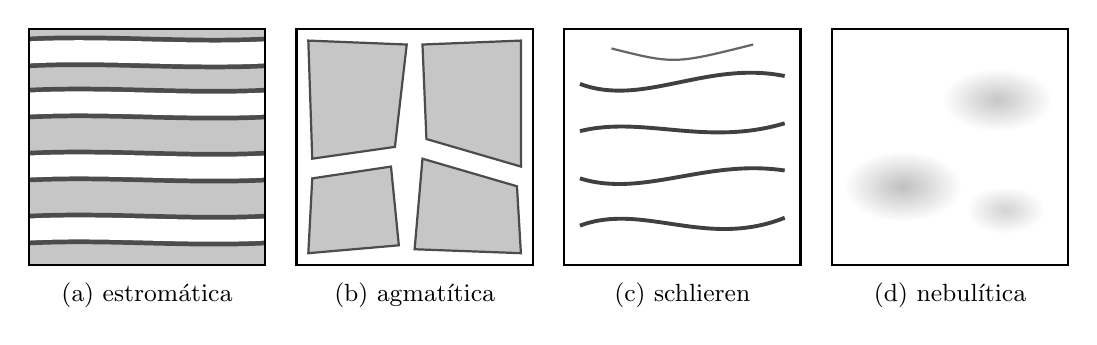
\begin{tikzpicture}[x=1cm, y=1cm]
% (a) stromatic
\begin{scope}
\fill[gray!45] (0,0) rectangle (3,3);
\foreach \y in {0.45, 1.25, 2.05, 2.7} {
  \fill[black!70] (0,\y-0.2) .. controls (1,\y-0.15) and (2,\y-0.25) .. (3,\y-0.2)
    -- (3,\y+0.2) .. controls (2,\y+0.15) and (1,\y+0.25) .. (0,\y+0.2) -- cycle;
  \fill[white] (0,\y-0.14) .. controls (1,\y-0.09) and (2,\y-0.19) .. (3,\y-0.14)
    -- (3,\y+0.14) .. controls (2,\y+0.09) and (1,\y+0.19) .. (0,\y+0.14) -- cycle;
}
\draw[thick] (0,0) rectangle (3,3);
\node[font=\small, anchor=north] at (1.5,-0.1) {(a) estromática};
\end{scope}
% (b) agmatitic
\begin{scope}[xshift=3.4cm]
\fill[white] (0,0) rectangle (3,3);
\fill[gray!45, draw=black!70, thick] (0.15,0.15) -- (1.3,0.25) -- (1.2,1.25) -- (0.2,1.1) -- cycle;
\fill[gray!45, draw=black!70, thick] (1.5,0.2) -- (2.85,0.15) -- (2.8,1.0) -- (1.6,1.35) -- cycle;
\fill[gray!45, draw=black!70, thick] (0.2,1.35) -- (1.25,1.5) -- (1.4,2.8) -- (0.15,2.85) -- cycle;
\fill[gray!45, draw=black!70, thick] (1.65,1.6) -- (2.85,1.25) -- (2.85,2.85) -- (1.6,2.8) -- cycle;
\draw[thick] (0,0) rectangle (3,3);
\node[font=\small, anchor=north] at (1.5,-0.1) {(b) agmatítica};
\end{scope}
% (c) schlieric
\begin{scope}[xshift=6.8cm]
\fill[white] (0,0) rectangle (3,3);
\foreach \y/\a in {0.5/0.3, 1.1/-0.25, 1.7/0.2, 2.3/-0.3} {
  \draw[black!75, line width=1.4pt] (0.2,\y) .. controls (1,\y+\a) and (1.8,\y-\a) .. (2.8,\y+0.1);
}
\draw[black!60, line width=0.8pt] (0.6,2.75) .. controls (1.4,2.55) .. (2.4,2.8);
\draw[thick] (0,0) rectangle (3,3);
\node[font=\small, anchor=north] at (1.5,-0.1) {(c) schlieren};
\end{scope}
% (d) nebulitic
\begin{scope}[xshift=10.2cm]
\fill[white] (0,0) rectangle (3,3);
\shade[inner color=gray!50, outer color=white] (0.9,1.0) ellipse (0.75 and 0.45);
\shade[inner color=gray!45, outer color=white] (2.1,2.1) ellipse (0.7 and 0.4);
\shade[inner color=gray!35, outer color=white] (2.2,0.7) ellipse (0.5 and 0.3);
\draw[thick] (0,0) rectangle (3,3);
\node[font=\small, anchor=north] at (1.5,-0.1) {(d) nebulítica};
\end{scope}
\end{tikzpicture}
\par\smallskip{\small Quatro estruturas de \omterm{def:b2:crustal-melting:migmatite}{migmatitos}, esquemáticas (faces de afloramento com cerca de um metro
de largura). Branco: \omterm{def:b2:crustal-melting:migmatite}{leucossoma}; preto: \omterm{def:b2:crustal-melting:migmatite}{melanossoma}; cinza: mesossoma. (a) Estromática: camadas de
\omterm{def:b2:crustal-melting:migmatite}{leucossoma}, cada uma com uma orla escura, paralelas à foliação, típicas dos \omterm{def:b2:crustal-melting:migmatite}{metatexitos}.
(b) Agmatítica: uma rede de veios de \omterm{def:b2:crustal-melting:migmatite}{leucossoma} em torno de blocos angulosos, que dá um aspecto
brechado. (c) Schlieren: estrias de minerais escuros dentro do \omterm{def:b2:crustal-melting:migmatite}{leucossoma}. (d) Nebulítica: fantasmas
difusos da rocha anterior em uma matriz de aspecto ígneo; (c) e (d) são típicas dos
\omterm{def:b2:crustal-melting:migmatite}{diatexitos}.}
\end{omfigure}
% ledger: bgs99:migmatite, scmr:migmatite

\begin{omfigure}
\centering
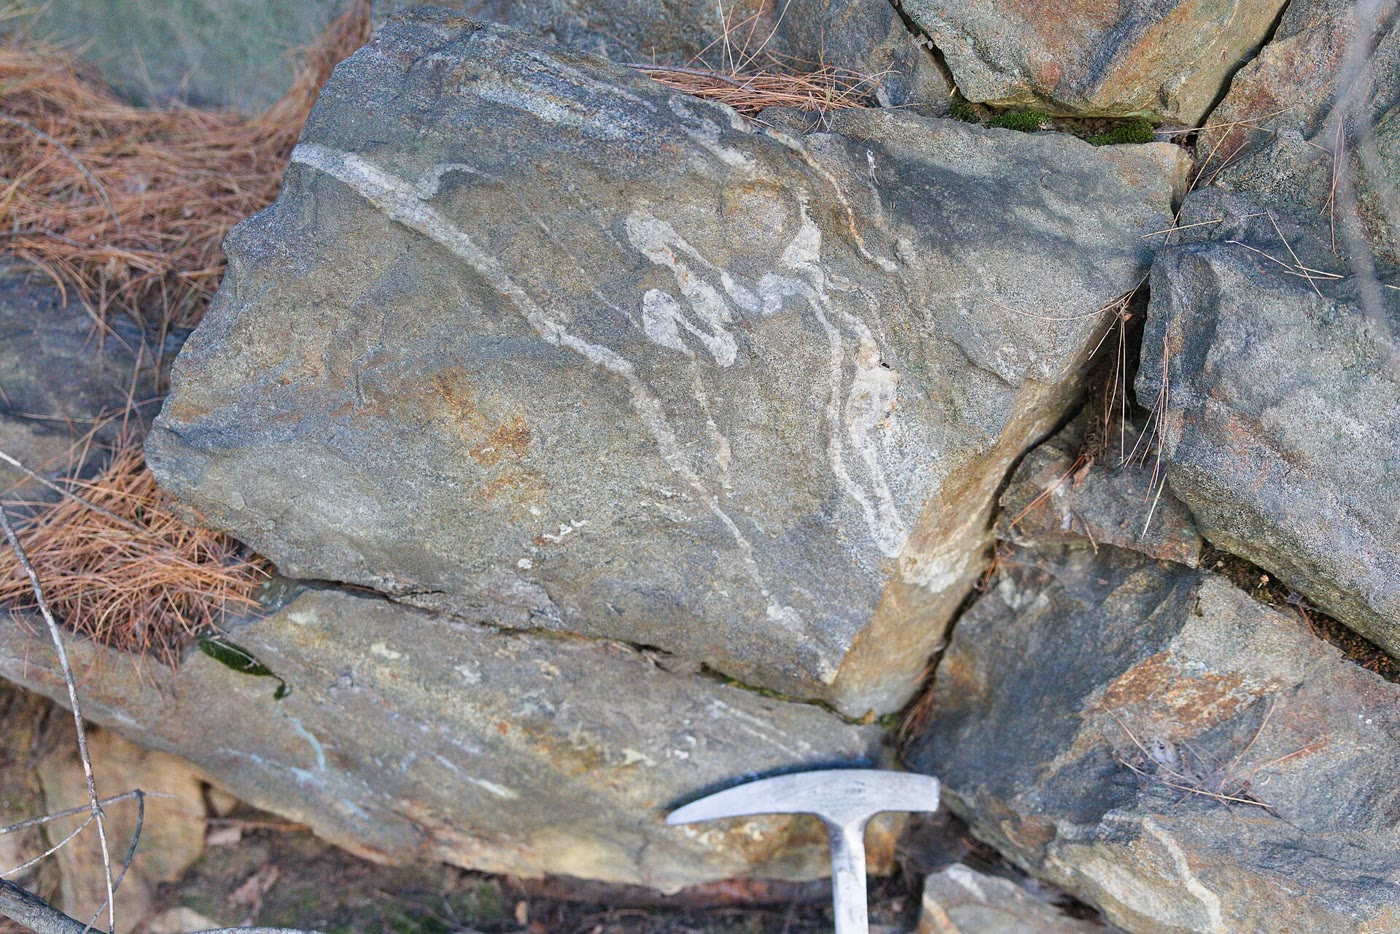
\includegraphics[width=0.62\linewidth]{images/book4/b2-12-migmatite.jpg}
\par\smallskip{\small Um \omterm{def:b2:crustal-melting:migmatite}{migmatito} em Nashua, New Hampshire: veios claros de \omterm{def:b2:crustal-melting:migmatite}{leucossoma}, dobrados
com o gnaisse cinza que os contém. O martelo do geólogo dá a escala. Fotografia de Kevin M. Gill, CC BY 4.0.}
\end{omfigure}

\section{Do migmatito ao plúton}\label{sec:b2:crustal-melting:segregation}

Na escala do grão, o primeiro fundido fica ao longo dos limites dos grãos e em pequenas bolsas,
em geral paralelas à foliação. Por pequeno que seja, ele muda a rocha: em experimentos com
granito parcialmente fundido, a resistência do agregado cai bruscamente entre o solidus
e uma \omterm{def:b2:mantle-melting:fraction}{fração de fundido} de \num{0.07}, à medida que os limites de grão com fundido se conectam, e volta a cair,
cerca de quatro ordens de grandeza, mas a partir de um valor já baixo, quando o arcabouço
cristalino se desfaz em \omterm{def:b2:mantle-melting:fraction}{frações de fundido} mais altas. A crosta parcialmente fundida é portanto fraca,
e a deformação se concentra ali assim que a fusão começa. A deformação, por sua vez, mobiliza o
fundido: ele drena da matriz ao longo de limites de grão interligados para \omterm{def:b2:crustal-melting:migmatite}{leucossomas} paralelos à
foliação, depois para fora da camada em fusão por \omterm{def:b2:crustal-melting:migmatite}{leucossomas} que a cortam, e
estes se juntam nos \omterm{def:b2:magma-emplacement:bodies}{diques} do \cref{ch:b2:magma-emplacement}. A figura abaixo resume o
caminho da fonte ao \omterm{def:b2:magma-emplacement:bodies}{plúton}.
% ledger: sawyer01:segregation, rh05:connectivity

\begin{omfigure}
\centering
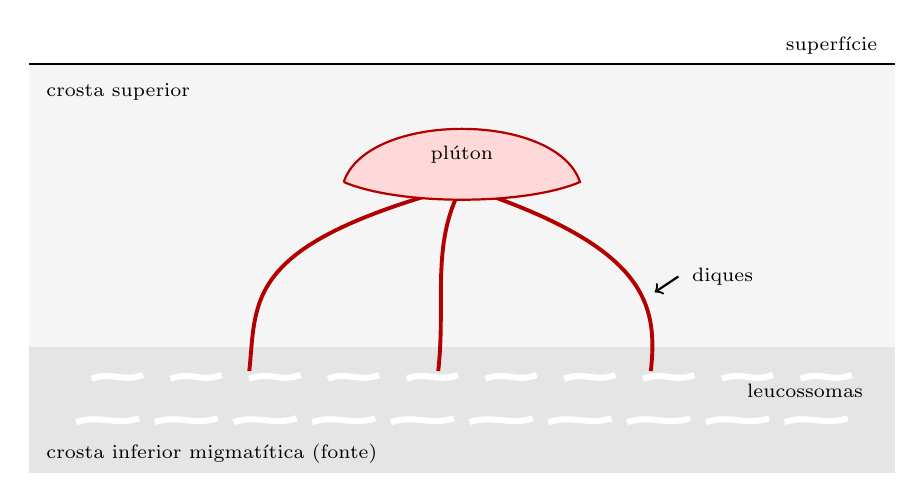
\begin{tikzpicture}[x=1cm, y=1cm]
\fill[gray!20] (0,0) rectangle (11,1.6);
\fill[gray!8] (0,1.6) rectangle (11,5.2);
\node[font=\scriptsize, anchor=west] at (0.1,0.25) {crosta inferior migmatítica (fonte)};
\foreach \x in {0.6,1.6,2.6,3.6,4.6,5.6,6.6,7.6,8.6,9.6} {
  \draw[white, line width=2.2pt] (\x,0.65) .. controls (\x+0.3,0.75) and (\x+0.5,0.6) .. (\x+0.8,0.7);
  \draw[white, line width=2.2pt] (\x+0.2,1.2) .. controls (\x+0.45,1.3) and (\x+0.6,1.15) .. (\x+0.85,1.25);
}
\foreach \x in {2.8, 5.2, 7.9} {
  \draw[red!70!black, line width=1.4pt] (\x,1.3) .. controls (\x+0.1,2.2) and (\x-0.1,2.9) .. (5.5,3.65);
}
\fill[pink!60, draw=red!70!black, thick] (4.0,3.7) .. controls (4.3,4.6) and (6.7,4.6) .. (7.0,3.7)
  .. controls (6.3,3.4) and (4.7,3.4) .. (4.0,3.7);
\node[font=\scriptsize] at (5.5,4.05) {plúton};
\node[font=\scriptsize, anchor=west] at (8.3,2.5) {diques};
\draw[->, thick] (8.25,2.5) -- (7.95,2.3);
\node[font=\scriptsize, anchor=west] at (0.1,4.85) {crosta superior};
\draw[thick] (0,5.2) -- (11,5.2);
\node[font=\scriptsize, anchor=south east] at (10.9,5.2) {superfície};
\node[font=\scriptsize, align=left, anchor=west] at (9.0,1.05) {leucossomas};
\end{tikzpicture}
\par\smallskip{\small Do \omterm{def:b2:crustal-melting:migmatite}{migmatito} ao \omterm{def:b2:magma-emplacement:bodies}{plúton}, esquemático e fora de escala: os \omterm{def:b2:crustal-melting:migmatite}{leucossomas}
(brancos) na fonte parcialmente fundida se juntam em \omterm{def:b2:magma-emplacement:bodies}{diques} (vermelho) que alimentam um \omterm{def:b2:magma-emplacement:bodies}{plúton} mais acima na
crosta.}
\end{omfigure}

Quanto tempo a crosta permanece fundida? No Himalaia, a \omterm{def:b2:crustal-melting:anatexis}{anatexia} generalizada começou cerca de
30 milhões de anos depois da colisão da Índia com a Ásia, e o zircão e a monazita das
rochas anatéticas dão idades de cerca de 25 a 15 milhões de anos atrás; uma única amostra pode cobrir
a maior parte desse intervalo. A fusão da crosta himalaiana não foi um evento, mas um estado que
durou cerca de dez milhões de anos.
% ledger: weinberg16:himalaya

\section{Tipos de granito}\label{sec:b2:crustal-melting:types}

Um granito se lembra de sua fonte em sua química, antes de tudo na quantidade de alumínio que
tem em comparação com o que seus feldspatos podem receber.

\begin{definition}[Índice de saturação em alumínio]\label{def:b2:crustal-melting:asi}
O \emph{índice de saturação em alumínio}\index{índice de saturação em alumínio} de uma rocha é a
razão molar
\[\mathrm{A/CNK} = \frac{n(\ce{Al2O3})}{n(\ce{CaO}) + n(\ce{Na2O}) + n(\ce{K2O})},\]
e seu índice companheiro é $\mathrm{A/NK} = n(\ce{Al2O3})/[n(\ce{Na2O}) + n(\ce{K2O})]$. Uma rocha
é \emph{peraluminosa}\index{peraluminoso} se $\mathrm{A/CNK} > 1$,
\emph{metaluminosa}\index{metaluminoso} se $\mathrm{A/CNK} < 1 < \mathrm{A/NK}$, e
\emph{peralcalina}\index{peralcalino} se $\mathrm{A/NK} < 1$.
\end{definition}
% ledger: moyen17:aluminosity, frost01:asi

\begin{proposition}[O que o índice mede]\label{prop:b2:crustal-melting:feldspar}
Uma rocha cujo cálcio, sódio e potássio estão todos em feldspatos, e cujo alumínio está
todo em feldspatos, tem $\mathrm{A/CNK} = 1$. Assim, uma rocha \omterm{def:b2:crustal-melting:asi}{peraluminosa} tem alumínio
sobrando depois de seus feldspatos, contido em minerais aluminosos (muscovita, granada, cordierita,
aluminossilicato); uma rocha \omterm{def:b2:crustal-melting:asi}{metaluminosa} tem cálcio sobrando, contido em silicatos de cálcio
(hornblenda, clinopiroxênio, titanita); e uma rocha \omterm{def:b2:crustal-melting:asi}{peralcalina} tem sódio e potássio
sobrando, contidos em minerais sem alumínio suficiente para o feldspato (piroxênio sódico e
anfibólio sódico).
\end{proposition}

\begin{proof}
Escritos na forma de óxidos, o feldspato potássico se torna \ce{K2O.Al2O3.6SiO2}, a albita se torna
\ce{Na2O.Al2O3.6SiO2} e a anortita, \ce{CaO.Al2O3.2SiO2}: cada fórmula tem exatamente um \ce{Al2O3} para um
\ce{K2O}, \ce{Na2O} ou \ce{CaO}. Qualquer mistura dos três tem portanto $n(\ce{Al2O3}) =
n(\ce{CaO}) + n(\ce{Na2O}) + n(\ce{K2O})$, isto é, $\mathrm{A/CNK} = 1$. Se
$\mathrm{A/CNK} > 1$, o alumínio excede o que os álcalis e o cálcio podem ligar em
feldspato, e o excesso deve ficar em outros minerais. Se $\mathrm{A/CNK} < 1$, mas
$\mathrm{A/NK} > 1$, há alumínio suficiente para todo o sódio e o potássio na forma de
feldspato, mas não para todo o cálcio, que vai para minerais que precisam de menos alumínio
por cálcio que a anortita. Se $\mathrm{A/NK} < 1$, nem mesmo os álcalis podem estar todos em
feldspato.
\end{proof}

Moyen e colaboradores consideraram a aluminosidade o indicador mais útil para distinguir granitos
de fontes diferentes; Frost e colaboradores usam o mesmo índice, com uma pequena
correção para o fósforo, como um dos três eixos de sua classificação das rochas
graníticas.
% ledger: moyen17:aluminosity, frost01:asi

\begin{omfigure}
\centering
\begin{tikzpicture}
\begin{axis}[omrecord, width=0.72\linewidth, height=7cm,
  xmin=0.4, xmax=1.5, ymin=0.4, ymax=3.5, xlabel={A/CNK (molar)}, ylabel={A/NK (molar)},
  tick label style={font=\scriptsize}, label style={font=\small}]
\addplot[fill=gray!15, draw=none] coordinates {(0.4,0.4) (1.5,1.5) (1.5,0.4) (0.4,0.4)};
\addplot[thick, black!70] coordinates {(1,0.4) (1,3.5)};
\addplot[thick, black!70] coordinates {(0.4,1) (1.5,1)};
\node[font=\scriptsize, anchor=north east] at (axis cs:1.48,3.45) {peraluminoso};
\node[font=\scriptsize, anchor=west] at (axis cs:0.62,2.6) {metaluminoso};
\node[font=\scriptsize, anchor=south west] at (axis cs:0.42,0.45) {peralcalino};
\addplot[only marks, mark=*, mark size=2pt, blue!70!black, nodes near coords,
  point meta=explicit symbolic, every node near coord/.style={font=\scriptsize, anchor=west}]
  coordinates {(0.539,3.196)[BHVO-2] (0.877,1.694)[AGV-2] (0.993,1.135)[SRM 278]};
\addplot[only marks, mark=square*, mark size=2pt, red!70!black]
  coordinates {(1.261,1.377) (0.809,0.844)};
\node[font=\scriptsize, red!70!black, anchor=south] at (axis cs:1.261,1.45) {fundido tipo S};
\node[font=\scriptsize, red!70!black, anchor=north] at (axis cs:0.809,0.79) {granito peralcalino};
\end{axis}
\end{tikzpicture}
\par\smallskip{\small O diagrama de Shand. Círculos azuis: três materiais de referência, um basalto
havaiano (BHVO-2), um andesito (AGV-2) e uma obsidiana de composição granítica (SRM 278),
calculados a partir de seus teores de óxidos publicados. Quadrados vermelhos: dois granitos inventados usados
neste capítulo. O triângulo cinza é inatingível, já que A/CNK nunca excede A/NK.}
\end{omfigure}
% ledger: usgs:bhvo2-major, usgs:agv2-major, nist278:majors

A química segue a fonte. Em 1974, Chappell e White notaram que, à parte as rochas
mais félsicas, os granitos do Cinturão Dobrado de Lachlan se dividem em dois grupos distintos,
e os interpretaram como fundidos de dois tipos de rocha-fonte: rochas ígneas mais antigas e rochas sedimentares. A hidrólise dos feldspatos, vista no volume do primeiro
ano, leva o sódio e o cálcio embora em solução e conserva o alumínio nas argilas: as lamas feitas
dessas argilas são ricas em alumínio, assim como seus fundidos.
% ledger: cw01:is-types

\begin{definition}[Tipologia dos granitos]\label{def:b2:crustal-melting:types}
Um \emph{granito tipo I}\index{granito tipo I} é um granito cuja fonte foi predominantemente uma
rocha ígnea mais antiga; um \emph{granito tipo S}\index{granito tipo S}, um granito cuja fonte foi
predominantemente uma rocha sedimentar (metassedimentar); e um granito tipo M, um granito derivado
do manto. Um \emph{granito tipo A}\index{granito tipo A} é definido por sua química e por seu
contexto, e não por sua fonte: ferroso e potássico, fortemente enriquecido em \omterm{def:b2:elements-in-the-earth:partition}{elementos incompatíveis},
e alojado em contextos intraplaca estáveis, de retroarco ou pós-colisionais.
\end{definition}
% ledger: johansson23:a-type, cw01:is-types

Os \omterm{def:b2:crustal-melting:types}{granitos tipo S} são \omterm{def:b2:crustal-melting:asi}{peraluminosos}, com duas micas ou com cordierita; os granitoides tipo A
são em sua maioria \omterm{def:b2:crustal-melting:asi}{metaluminosos}, alguns \omterm{def:b2:crustal-melting:asi}{peraluminosos}. Uma única análise pode enganar, porém: toda
suíte de granitoides termina perto da composição do mínimo granítico, leucocrática e ligeiramente
\omterm{def:b2:crustal-melting:asi}{peraluminosa}, de modo que uma amostra \omterm{def:b2:crustal-melting:asi}{peraluminosa} não prova que a crosta tenha fundido. O que distingue
as suítes é a forma de sua tendência no diagrama de Shand: uma suíte de arco chega ao
mínimo ao longo de um alinhamento íngreme vindo de A/NK alto e A/CNK baixo, uma suíte tipo S pobre em cálcio
ao longo de um alinhamento com A/NK próximo de A/CNK. Nenhum consenso foi alcançado sobre a fonte dos
\omterm{def:b2:magma-emplacement:magma}{magmas} tipo A: um modelo os produz a partir de basalto sobreplacado, evoluído por cristalização,
\omterm{def:b2:mantle-melting:melting}{fusão parcial} e assimilação de crosta.
% ledger: moyen17:trends, frost01:asi, johansson23:a-type

\begin{definition}[Leucogranito]\label{def:b2:crustal-melting:leucogranite}
Um \emph{leucogranito}\index{leucogranito} é um granito de cor clara, quase sem
minerais escuros; os leucogranitos \omterm{def:b2:crustal-melting:asi}{peraluminosos} dos cinturões de colisão contêm muscovita, sozinha ou
com biotita.
\end{definition}
% ledger: moyen17:aluminosity, pdh98:himalaya

Os \omterm{def:b2:crustal-melting:leucogranite}{leucogranitos} \omterm{def:b2:crustal-melting:asi}{peraluminosos} a muscovita dos cinturões de colisão têm composições próximas
dos líquidos da fusão com água ou da \omterm{def:b2:crustal-melting:reactions}{fusão por desidratação} da muscovita, a temperaturas próximas de
\qty{700}{\celsius}, em que o zircão e a monazita da fonte podem sobreviver e ser carregados
para o fundido como xenocristais; os granitos \omterm{def:b2:crustal-melting:asi}{peraluminosos} a cordierita vêm da
decomposição, mais quente, da biotita, a 800 a \qty{850}{\celsius}. Os \omterm{def:b2:crustal-melting:leucogranite}{leucogranitos} do Himalaia,
com sua forte assinatura isotópica crustal, pertencem a essa família
(\cref{ch:b2:himalaya-andes}).
% ledger: moyen17:aluminosity, weinberg16:himalaya

\begin{omfigure}
\centering
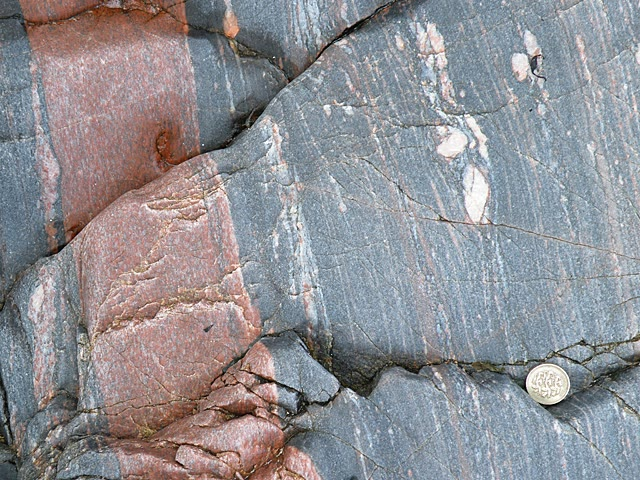
\includegraphics[width=0.5\linewidth]{images/book4/b2-12-leucogranite-vein.jpg}
\par\smallskip{\small Um veio de \omterm{def:b2:crustal-melting:leucogranite}{leucogranito} rosa cortando um gnaisse cinza bandado; a moeda dá
a escala. Fotografia de Anne Burgess (Geograph), CC BY-SA 2.0.}
\end{omfigure}

\section{Os granitos e o crescimento dos continentes}\label{sec:b2:crustal-melting:time}

Dois tipos de lugares produzem a maior parte do granito. Acima das zonas de subducção, a crosta de arco se forma pela
diferenciação de fundidos máficos vindos do manto, e o calor disponível é apenas o que esses
fundidos trazem. Depois de uma colisão, a crosta espessada é um sistema muito quente: ela funde em
grande escala, a baixa temperatura onde a água ou a muscovita o permitem e a temperatura mais
alta pela decomposição da biotita, e esses granitos de origem crustal reciclam uma crosta que
já existia. Os fundidos mantélicos também chegam à crosta ali, em quantidades grandes o bastante, segundo Moyen e
colaboradores, para fazer dos cinturões tardiorogênicos contribuintes importantes para o crescimento da
crosta. Se um granito acrescenta aos continentes ou apenas os retrabalha é portanto uma questão de
sua fonte, à qual seus isótopos respondem (\cref{ch:b2:isotope-geochemistry}); os granitos da
Terra primitiva, muito diferentes destes, são o assunto do
\cref{ch:b2:precambrian-earth}.
% ledger: moyen17:settings

\section{Exercícios}\label{sec:b2:crustal-melting:exercises}

Massas molares (\unit{\gram\per\mole}): \ce{Al2O3} 101.96, \ce{CaO} 56.08, \ce{Na2O} 61.98,
\ce{K2O} 94.20, \ce{H2O} 18.02; massas atômicas: H 1.008, O 16.00, Na 22.99, Mg 24.31,
Al 26.98, Si 28.09, K 39.10, Ca 40.08. Tome $g = \qty{9.81}{\metre\per\second\squared}$.

\begin{exercise}[$\star$]\label{exo:b2:crustal-melting:1}
O material de referência andesítico AGV-2 contém, em \unit{\gram} por \qty{100}{\gram},
\ce{Al2O3} 17.03, \ce{CaO} 5.15, \ce{Na2O} 4.204 e \ce{K2O} 2.898.
(a) Calcule seus A/CNK e A/NK. (b) Classifique-o, e dê um mineral que deveria conter seu
excesso de cálcio.
\end{exercise}
% ledger: usgs:agv2-major

\begin{exercise}[$\star$]\label{exo:b2:crustal-melting:2}
Três granitos contêm, além de quartzo e feldspatos: (a) muscovita, biotita e granada;
(b) hornblenda, biotita e titanita; (c) egirina, um piroxênio de sódio e ferro
\ce{NaFeSi2O6}, e um anfibólio sódico. Classifique cada um por sua saturação em alumínio, e diga
qual poderia ser um \omterm{def:b2:crustal-melting:types}{granito tipo S}.
\end{exercise}

\begin{exercise}[$\star$]\label{exo:b2:crustal-melting:3}
Uma crosta de densidade \qty{2800}{\kilogram\per\cubic\metre} tem uma geoterma linear
$T = \qty{10}{\celsius} + (\qty{20}{\celsius\per\kilo\metre})\,z$. Entre 2 e
\qty{10}{kbar}, aproxime o solidus úmido do granito pela reta que passa por
(\qty{680}{\celsius}, \qty{2}{kbar}) e (\qty{620}{\celsius}, \qty{10}{kbar}). A que
profundidade, temperatura e pressão a geoterma o encontra?
\end{exercise}
% ledger: sw81:wet-solidus

\begin{exercise}[$\star$]\label{exo:b2:crustal-melting:4}
Um gnaisse cinza a biotita contém camadas brancas de quartzo e feldspato, de um centímetro de espessura, paralelas
à sua foliação, cada uma orlada por uma fina faixa negra de biotita; entre as camadas, o
gnaisse parece comum. (a) Dê o nome das camadas brancas, das faixas negras e do gnaisse comum.
(b) A rocha é um \omterm{def:b2:crustal-melting:migmatite}{metatexito} ou um \omterm{def:b2:crustal-melting:migmatite}{diatexito}, e qual é sua estrutura? (c) Algumas centenas de
metros adiante, o bandamento desapareceu: uma rocha estriada, de aspecto granítico, contém tênues fantasmas de
gnaisse. O que mudou?
\end{exercise}
% ledger: scmr:migmatite, bgs99:migmatite

\begin{exercise}[$\star\star$]\label{exo:b2:crustal-melting:5}
Tome a biotita como flogopita, \ce{KMg3AlSi3O10(OH)2}. (a) Calcule sua massa molar e a
fração em massa de água que ela libera (seus dois grupos hidroxila dão um \ce{H2O}).
(b) Um gnaisse com \qty{25}{\percent} de biotita em massa funde por desidratação da biotita
gerando um fundido com \qty{4.0}{\percent} de água. Usando a
\cref{prop:b2:crustal-melting:water}, encontre a \omterm{def:b2:mantle-melting:fraction}{fração de fundido}, e compare-a com as
frações encontradas em experimentos de \omterm{def:b2:crustal-melting:reactions}{fusão por desidratação} da biotita.
\end{exercise}
% ledger: bk99:migmatites

\begin{exercise}[$\star\star$]\label{exo:b2:crustal-melting:6}
Cem gramas de granito contêm \qty{30}{\gram} de feldspato potássico \ce{KAlSi3O8},
\qty{35}{\gram} de albita \ce{NaAlSi3O8}, \qty{5}{\gram} de anortita \ce{CaAl2Si2O8},
\qty{25}{\gram} de quartzo e \qty{5}{\gram} de muscovita \ce{KAl3Si3O10(OH)2}.
(a) Calcule as massas molares dos quatro minerais aluminosos. (b) Calcule as quantidades de
\ce{Al2O3}, \ce{CaO}, \ce{Na2O} e \ce{K2O} na rocha, e seu A/CNK. (c) Que
mineral torna a rocha \omterm{def:b2:crustal-melting:asi}{peraluminosa}?
\end{exercise}

\begin{exercise}[$\star\star$]\label{exo:b2:crustal-melting:7}
Uma \omterm{def:b2:magma-emplacement:bodies}{soleira} basáltica intrudida a \qty{1200}{\celsius} cristaliza completamente e se resfria até
\qty{850}{\celsius}, liberando um calor latente de \qty{900}{\mega\joule\per\cubic\metre}.
A crosta ao seu redor, a \qty{650}{\celsius}, é aquecida até \qty{850}{\celsius} e
\qty{20}{\percent} dela funde, com o mesmo calor latente por unidade de volume de fundido. As duas
rochas têm uma capacidade térmica de \qty{2.5}{\mega\joule\per\cubic\metre\per\kelvin}. Usando a
\cref{prop:b2:crustal-melting:heat}, quantos metros cúbicos de crosta um metro cúbico
de basalto pode tratar assim? O que o resultado ignora?
\end{exercise}
% ledger: delaney86b4:properties

\begin{exercise}[$\star\star$]\label{exo:b2:crustal-melting:8}
O material de referência obsidiana SRM 278 é certificado em \ce{Al2O3}
$14.15 \pm 0.15$, \ce{CaO} 0.983, \ce{Na2O} 4.84 e \ce{K2O} 4.16 (\unit{\percent} em
massa). (a) Calcule seus A/CNK e A/NK e classifique-o. (b) Recalcule A/CNK com os dois
extremos da incerteza de \ce{Al2O3}. A classificação é robusta?
\end{exercise}
% ledger: nist278:majors

\begin{exercise}[$\star\star$]\label{exo:b2:crustal-melting:9}
A \qty{800}{\celsius}, um fundido haplogranítico saturado em água contém \qty{7.45}{\percent}
de água a \qty{3}{kbar}, 8.94 a \qty{4}{kbar}, 9.97 a \qty{5}{kbar} e 13.82 a
\qty{8}{kbar}. (a) Ajuste uma reta a esses quatro pontos por mínimos quadrados e compare
sua inclinação com os \qty{1.27}{\percent} por quilobar indicados pelos experimentadores.
(b) Preveja o teor de saturação a \qty{6}{kbar}. (c) Qual é a menor massa de fundido
que pode carregar \qty{10}{\gram} de água a \qty{6}{kbar}? (d) Por que a reta não deve ser
usada a \qty{15}{kbar}?
\end{exercise}
% ledger: holtz95:solubility

\begin{exercise}[$\star\star\star$]\label{exo:b2:crustal-melting:10}
Aproxime o solidus de \omterm{def:b2:crustal-melting:reactions}{fusão por desidratação} de um muscovita-xisto pela reta que passa
por (\qty{750}{\celsius}, \qty{6}{kbar}) e (\qty{800}{\celsius}, \qty{10}{kbar}),
os extremos dos intervalos experimentais. Um xisto a \qty{770}{\celsius} sobe a partir de
\qty{10}{kbar} sem ganhar nem perder calor. (a) A que pressão ele atinge o
solidus? (b) Além dela, sua temperatura segue o solidus para baixo, e o calor da fusão vem
de seu próprio resfriamento. Com uma capacidade térmica de \qty{2.5}{\mega\joule\per\cubic\metre\per\kelvin}
e um calor latente de \qty{900}{\mega\joule\per\cubic\metre}, que fração em volume de fundido
se formou quando ele chega a \qty{6}{kbar}? (c) Compare com as condições propostas para os
\omterm{def:b2:crustal-melting:leucogranite}{leucogranitos} do Himalaia.
\end{exercise}
% ledger: pdh98:himalaya, delaney86b4:properties

\begin{exercise}[$\star\star\star$]\label{exo:b2:crustal-melting:11}
O calor se difunde por uma distância $\ell$ em um tempo da ordem de $\ell^2/\kappa$. Com
$\kappa = \qty{1e-6}{\square\metre\per\second}$, estime o tempo para que o calor de uma
\omterm{def:b2:magma-emplacement:bodies}{soleira} de \qty{2}{km} de espessura, e de uma camada sobreplacada de \qty{10}{km} de espessura, se espalhe por sua
própria espessura. Compare com os dez milhões de anos da \omterm{def:b2:crustal-melting:anatexis}{anatexia} himalaiana: um único
evento de sobreplacamento pode explicá-la?
\end{exercise}
% ledger: delaney86b4:properties, weinberg16:himalaya

\begin{exercise}[$\star\star\star$]\label{exo:b2:crustal-melting:12}
Um \omterm{def:b2:crustal-melting:migmatite}{migmatito} estromático é analisado: \omterm{def:b2:crustal-melting:migmatite}{leucossoma} \ce{K2O} \qty{5.0}{\percent}, \ce{MgO}
\qty{0.20}{\percent}; \omterm{def:b2:crustal-melting:migmatite}{melanossoma} \ce{K2O} \qty{2.0}{\percent}, \ce{MgO}
\qty{4.0}{\percent}; mesossoma, tomado como a rocha original não fundida, \ce{K2O}
\qty{2.75}{\percent}, \ce{MgO} \qty{3.05}{\percent} (tudo em massa). (a) Se o
neossoma se formou a partir da rocha original sem ganho nem perda, que fração em massa dele é
\omterm{def:b2:crustal-melting:migmatite}{leucossoma}? (b) Verifique a resposta com \ce{MgO}. (c) No afloramento, o \omterm{def:b2:crustal-melting:migmatite}{leucossoma} representa apenas
\qty{10}{\percent} do neossoma em massa. Quantos gramas de fundido saíram por
\qty{100}{\gram} de rocha original?
\end{exercise}

\begin{problem}[{Problema de fim de semana --- um plúton a partir de mica fundida}]\label{pb:b2:crustal-melting:1}
Um xisto formado de \qty{20}{\percent} de muscovita, \qty{15}{\percent} de biotita,
\qty{30}{\percent} de quartzo, \qty{30}{\percent} de plagioclásio e \qty{5}{\percent} de outros
minerais (em massa; uma rocha inventada) fica na base de uma crosta duplicada por empilhamento, a
situação modelada no \cref{ch:b2:pt-paths}. Ele pode fundir e alimentar um \omterm{def:b2:magma-emplacement:bodies}{plúton} granítico. Dados:
as massas atômicas e molares do início dos exercícios; o solidus úmido do granito passa
por (\qty{680}{\celsius}, \qty{2}{kbar}), (\qty{620}{\celsius}, \qty{10}{kbar}),
(\qty{605}{\celsius}, \qty{15.3}{kbar}) e (\qty{670}{\celsius}, \qty{27}{kbar}); o
teor de saturação em água de um fundido granítico a \qty{800}{\celsius} é de \qty{9.97}{\percent} a
\qty{5}{kbar} e \qty{13.82}{\percent} a \qty{8}{kbar}. A base modelo da crosta espessada segue:

\smallskip
\begin{center}\small
\begin{tabular}{l|ccccccccccc}
$t$ (\unit{Myr}) & 0 & 10 & 20 & 30 & 40 & 50 & 60 & 70 & 80 & 90 & 100\\ \hline
$T$ (\unit{\celsius}) & 595 & 656 & 734 & 795 & 845 & 885 & 909 & 914 & 900 & 867 & 814\\
$P$ (\unit{kbar}) & 19.2 & 19.2 & 19.2 & 19.2 & 17.9 & 16.5 & 15.1 & 13.7 & 12.4 & 11.0 & 9.6
\end{tabular}
\end{center}
\smallskip

\noindent\textbf{Parte I --- A água da mica.}
\begin{enumerate}
\item Calcule a massa molar da muscovita \ce{KAl3Si3O10(OH)2}.
\item Seus dois grupos hidroxila dão um \ce{H2O}. Que fração em massa do mineral é
liberada como água?
\item Quanta água a muscovita de um quilograma de xisto libera?
\item Interpolando linearmente, qual é o teor de água de saturação do fundido a
\qty{7}{kbar}? Qual é então a menor \omterm{def:b2:mantle-melting:fraction}{fração de fundido} que a água da muscovita pode produzir?
\item O fundido da \omterm{def:b2:crustal-melting:reactions}{fusão por desidratação} está longe da saturação; tome seu teor de água como
\qty{6.0}{\percent}. Que \omterm{def:b2:mantle-melting:fraction}{fração de fundido} a muscovita produz?
\item Em experimentos com um \omterm{def:b2:metamorphic-facies:protoliths}{metapelito} a duas micas a \qty{10}{kbar}, a reação da muscovita
deu apenas 1 a \qty{2}{\percent} de fundido. Dê duas razões pelas quais uma rocha real pode produzir menos
fundido que sua resposta à questão~5.
\end{enumerate}

\noindent\textbf{Parte II --- Aquecer a fonte.}
\begin{enumerate}[resume]
\item No \cref{ch:b2:pt-paths}, a rocha deixada a meia crosta tem seu pico a \qty{593}{\celsius}
e \qty{7.8}{kbar}. Qual é o solidus úmido a \qty{7.8}{kbar}? Essa rocha pode fundir, mesmo
com água livre?
\item Interpolando entre 15.3 e \qty{27}{kbar}, encontre o solidus úmido à pressão
da base logo depois do empilhamento. A base está acima dele em $t = 0$? Em $t = \qty{10}{Myr}$?
\item O que limita a fusão da base em $t = \qty{10}{Myr}$, e por que ela para
logo?
\item Quando a base passa de \qty{800}{\celsius}, o extremo superior do intervalo da
muscovita?
\item O intervalo do anfibólio vai de 875 a \qty{925}{\celsius} a 10 a \qty{12.5}{kbar}.
Quando a base entra nessa faixa de pressão, e a que temperatura?
\item Quando a base chega a \qty{10}{kbar}, o topo da faixa de pressão dos
experimentos com muscovita, e quão quente ela está então? Que minerais hidratados do xisto podem
ainda existir?
\end{enumerate}

\noindent\textbf{Parte III --- Que fundido?}
O fundido, uma vez cristalizado, dá um \omterm{def:b2:crustal-melting:leucogranite}{leucogranito} (análise inventada) com, em
\unit{\percent} em massa, \ce{Al2O3} 15.0, \ce{CaO} 0.55, \ce{Na2O} 3.4 e \ce{K2O} 4.9.
\begin{enumerate}[resume]
\item Calcule as quantidades dos quatro óxidos em \qty{100}{\gram} da rocha.
\item Calcule seu A/CNK.
\item Calcule seu A/NK e classifique o \omterm{def:b2:crustal-melting:leucogranite}{leucogranito}.
\item Ele é um \omterm{def:b2:crustal-melting:types}{granito tipo I} ou tipo S? Dê dois minerais que deveriam conter seu excesso
de alumínio.
\item Quantos mols de \ce{Al2O3} por \qty{100}{\gram} sobram depois dos
feldspatos? Se todo ele fosse para a muscovita, que contém um \ce{Al2O3} a mais por unidade de
fórmula que o feldspato potássico, quantos gramas de muscovita \qty{100}{\gram} de granito
conteriam?
\item A obsidiana SRM 278 tem A/CNK $= 0.993$. O \omterm{def:b2:crustal-melting:leucogranite}{leucogranito} e a obsidiana poderiam
vir do mesmo tipo de fonte?
\end{enumerate}

\noindent\textbf{Parte IV --- Quanta crosta?}
Um \omterm{def:b2:magma-emplacement:bodies}{plúton} inventado desse \omterm{def:b2:crustal-melting:leucogranite}{leucogranito} tem um volume de \qty{1000}{\cubic\kilo\metre}.
Tome \qty{2650}{\kilogram\per\cubic\metre} para o granito e
\qty{2800}{\kilogram\per\cubic\metre} para o xisto; suponha que \qty{70}{\percent} do
fundido deixe sua fonte e que toda a água do fundido escape quando ele cristaliza.
\begin{enumerate}[resume]
\item Qual é a massa do \omterm{def:b2:magma-emplacement:bodies}{plúton}?
\item Que massa de fundido (com seus \qty{6.0}{\percent} de água) ele exigiu?
\item Usando a \omterm{def:b2:mantle-melting:fraction}{fração de fundido} da questão~5, que massa de xisto teve de fundir?
\item Que volume de xisto é esse?
\item Se a fonte era uma camada de \qty{5}{km} de espessura, sobre que área ela fundiu?
\item Com a menor \omterm{def:b2:mantle-melting:fraction}{fração de fundido} da questão~4, quanto maior seria a
fonte? Dê o volume de crosta-fonte fundida para produzir o \omterm{def:b2:magma-emplacement:bodies}{plúton}, em
\unit{\cubic\kilo\metre}, a partir da questão~22.
\end{enumerate}
\end{problem}
